\documentclass[12pt]{article}
%بسم الله الرحمن الرحیم

%You should edit DSLecture.tex, not this file!
\usepackage{amsthm}
\usepackage{latexsym}
\usepackage{amssymb}
\usepackage{verbatim}
\usepackage{enumitem,amsmath,array}
\usepackage{tikz}
\usepackage{tkz-graph}
\usepackage{bookmark}
\usetikzlibrary{positioning,chains,fit,shapes,calc}
\usepackage[a4paper, margin=0.7in]{geometry}
\usepackage{listings}
\usepackage{clrscode3e}
\usepackage{hyperref}
\hypersetup{
	colorlinks=true,
	linkcolor=blue,
	filecolor=magenta,
	urlcolor=cyan,
}
\usepackage[fontsloadable]{xepersian}


\settextfont{HM XNiloofar}
%\setdigitfont{HM XNiloofar}
%\setdigitfont{ParsiDigits}
\defpersianfont\outline[Scale=1]{HM XNiloofar Outline}

\setlength{\parindent}{1.5em}
\setlength{\parskip}{0.9em}
\renewcommand{\baselinestretch}{1.4}


\newcommand{\lecture}[3]{
	%\pagestyle{empty}
	{
			\begin{center}
				\vspace{-1cm}
				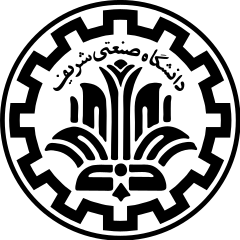
\includegraphics[scale=0.15]{Sharif}%\hfill \\[1em]  
			\end{center}
			\vspace{-8mm}
			\begin{center}

				\bf
				%\begin{outline} 
				{
					\Large
					مباحث ویژه در سیستم‌های دیجیتال
				}
				%\end{outline} 
				\\
				%مدرس: مرتضی علیمی
				%\\
				مدرس : دکتر ایمان غلامی
				\\~
				[پاییز 1400]
			\end{center}
		}\vspace*{-1em}
	\noindent
	تمرن سری #1 #2 \hfill نگارنده: #3
	\vspace{-4mm}
	\rule{\textwidth}{1pt}
	\ \\
}
\newcommand{\obligation}[1] {
\textbf{اینجانب #1 تعهد می‌دهم که  در نوشتن این تمرینات هیچگونه استفاده‌ای از منابع سال‌های گذشته نکرده‌ام، از مکتوبات هیچ فردی بهره نگرفته‌ام و همکاری بنده با دیگران در حد بحث و گفتگو و حل مسایل بوده‌است.}
\\
}

% example environment
\newenvironment{example}
{\smallskip \noindent \emph{مثال:}}
{\hfill $\boxtimes$ \smallskip}


\newtheorem{theorem}{قضیه}
\newtheorem{proposition}{گزاره}
\newtheorem{claim}{ادعا}
\newtheorem{lemma}{لم}
\newtheorem{corollary}{نتیجه}
\newtheorem{definition}{تعریف} % Use this for non-trivial definitions.

%%%%%%%%%%%%%%%%%%%%%%%%%%%%%%%%%%%%%%%%%%%%%%%%%%%%%%%%%%%%%%%%%%%%%%%%%%%%


\usepackage{graphicx}
\usepackage{commath}
\usetikzlibrary{arrows,automata}
\usetikzlibrary{circuits.logic.US}
\usepackage{tikz}
\usepackage{amsmath}
\usepackage{graphics}
\usepackage{pgfplots}
\pgfplotsset{width=7cm, compat=1.9}
\usepgfplotslibrary{fillbetween}
\usetikzlibrary{automata, positioning, arrows}
\begin{document}
\graphicspath{ {./} }
\lecture{5}{}{امیرمحمد شعبانی }
\section*{مقدمه}
سلام. در ابتدا تشکر ویژه‌ای برای آموزش مطالب جالب و کاربردی می‌کنم.
امیدوارم درس داده‌های حجیم در سال‌های آینده برای بچه‌های ورودی جدید نیز ارائه شود تا از آن بهره ببرند.

در ادامه روند کلی را توضیح می‌دهم و سپس سعی خود را می‌کنم که هربخش را با جزییات کامل و تمام چالش‌هایی که وجود داشت توضیح دهم.
پس از نصب ملزمات و لود کردن تمام فایل‌ها، سعی کردم با کمی
کند و کاو چند نمودار و کمی شهود از داده‌ها بدست بیاورم که بعضی نتایج جالب بودند.
سپس سعی کردم بعضی از الگوریتم‌هایی که در طول درس یاد گرفته‌ایم را روی داده‌ها پیاده‌سازی کنم و نتایج را خروجی دهم.
اگر چه در پیاده‌سازی بعضی از الگوریتم‌ها ناموفق بودم و یا با وجود پیاده‌سازی درست، در بدست‌آوردن نتیجه مناسب ناموفق بودم.

همچنین  در روند پروژه مشورت‌هایی با خانم ساحل مس‌فروش در مورد روند پیاده‌سازی و 
مخصوصا پیش‌پردازش‌های داده‌های ترافیک و پیدا‌کردن 
\lr{outliers}
کرده‌ایم.


\section*{نصب}
تنها نیازمندی جدی نصب 
\lr{pyspark}
خواهد بود که در ابتدای برنامه نصب می‌کنیم.
البته برای نمایش درست متون فارسی دو کتاب‌هانه دیگر را نصب می‌کنیم و زمان کشیدن نمودار‌ها متن‌ها را با آن‌ها تغییر می‌دهیم.

\subsection*{راه‌اندازی با کولب}
بخشی از کد‌ها که برای استخراج داده از درایو و یا وصل شدن به درایو است برای کسانی است که در کولب قصد اجرا آن را دارند.
همچنین اگر فایل‌ها در آدرس خاصی قرار دارد کافیست
\lr{base\_pass}
را ویرایش کنید و زمان لود فایل‌ها به ابتدای آدرس این متغیر را اضافه کنید.

\section*{راه‌اندازی اسپارک و لود فایل‌ها}
اسپارک را روی لوکال می‌سازیم و سپس 
\lr{schema}
ترافیک را از روی فایل آن درست می‌کنیم و سپس داده ترافیک را لود می‌کنیم. همچنین برای داده‌های
شرکت‌ها و سیستم‌ها و راستی‌آزمایی وضعیت همین کار را اجرا می‌کنیم. برای بخش‌هایی که با خط تیره داده‌ها را جدا کرده‌است،
آن‌ها را به آرایه تبدیل می‌کنیم.

\section*{پیش‌پردازش روی داده‌ها و بدست‌آوردن اطلاعات}
\subsection*{هرشرکت روی چند سیستم دوربین متفاوت کار می‌کند؟}
هر‌دوربین برای کار متفاوت ساخته شده‌است. بعضی از آن‌ها برای طرح زوج و فرد و بعضی برای چراغ‌های راهنمایی‌و‌رانندگی و 
$\dots$
هستند.


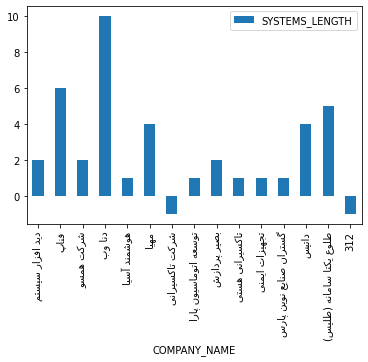
\includegraphics[scale=1]{companyLength.png}

\subsection*{چند شرکت متفاوت روی هر‌سیستم کار می‌کند؟}

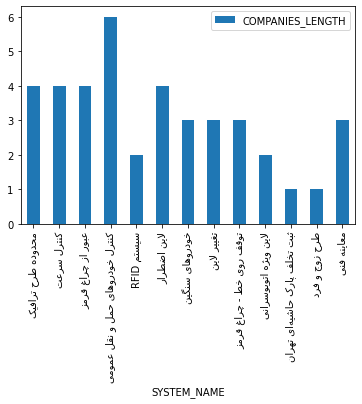
\includegraphics[scale=1]{systemLength.png}

\subsection*{هر‌شرکت چند‌بار نتوانست به صورت اتوماتیک پلاک‌ها را تشخیص دهد؟}
اگر وضعیت پلاک یک ماشین ۵ یا ۶ باشد آنگاه آن پلاک به صورت اتوماتیک بدست آمده‌است. بنابراین با فیلتر آن‌ها باقی پلاک‌ها یا درست تشخیص داده‌نشده‌اند و یا دستی بدست آمده‌است.

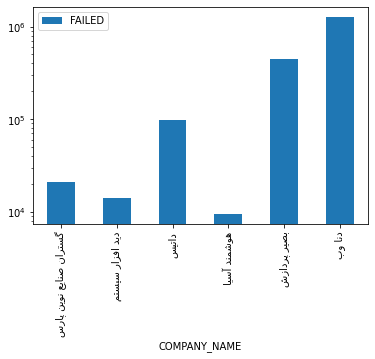
\includegraphics[scale=1]{faieldCompanies.png}

\subsection*{نرخ موفقیت دوربین‌ها در تشخیص درست یا غلط چقدر است؟}
با کمی حساب و کتاب می‌بینیم هم دوربین‌هایی وجود دارند که کاملا درست تشخیص داده‌اند و هم  دوربین‌هایی وجود دارند که نتوانستند درست تشخیص بدهند.
معیار تشخیص را دوربین‌هایی می‌گذاریم که نه به صورت اتوماتیک و نه به صورت دستی 
پلاکشان رهگیری نشده‌است. سپس تمام آن‌هایی نرخ تشخیص درستی پلاک آن‌ها از 
60 درصد کمتر باشد را از داده‌ها حذف می‌کنیم.

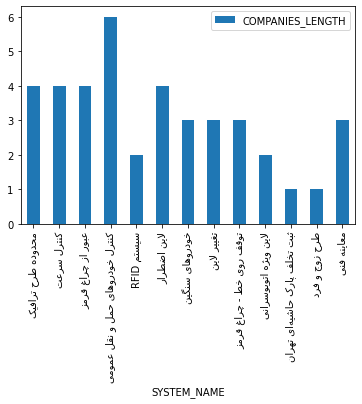
\includegraphics[scale=1]{systemLength.png}

\subsection*{حذف داده‌های پرت}
در بخش قبل بخشی از دوربین‌ها را دور انداختیم و حالا نوبت پاک‌سازی بهتر و درست‌تر نسبت به داده‌هایی که داریم است.

\subsubsection{پلاک‌هایی که زیاد دیده‌شده‌اند و غیر‌واقعی‌اند}
وقتی خلاصه‌ای از داده‌ها را نمایش دادیم میانگین دیده‌شدن هر پلاک به تقریب ۶ بار بوده‌است، اما
داده‌های کمی وجود داشته‌اند که بیش‌تر از ۱۰ هزار بار دیده‌شده‌اند.
احتمالا پلاک خودکاری است که دوربین‌ها پس از عدم تشخیص پلاک ثبت می‌کنند. همچنین
با ایمیل از شما نیز پرسیدیم و تایید کردید. بنابراین تصمیم گرفتم
چنین پلاک‌هایی را حذف کنم و تصمیم بر این شد پلاک‌هایی که کمتر از ۱۰۰ بار دیده‌شده‌اند را نگه دارم. این تصمیم را با 
دیدن داده‌ها و با احتساب اینکه تنها برای ۸ روز است انتخاب کردم. همچنین راه مناسب دیگر این است که 
چارک اول و سوم را محاسبه کنم و یک بازه منماسب با استفاده از آن‌ها بسازم و تنها پلاک‌هایی که به همان تعداد دیده‌شده‌اند را بگیرم.

\subsection*{بدست آوردن پلاک‌ها و دوبین‌های پرتردد}
کافیست یک بار براساس پلاک و بار دیگر براساس دوبین تعداد بار دیده‌شدن را بشماریم و سپس
با کشیدن هیستوگرام آن پرتردد ها را تشخیص دهیم و سپس فیلر کنیم.
پلاک‌هایی که بیشتر از ۷ بار دیده‌اند پرتردد محسوب می‌شوند و دوبین‌هایی که 
بیشتر از ۸۰ هزار ریکورد دارند را پرتردد می‌نامیم.

هیستوگرام شمارش دوربین‌ها

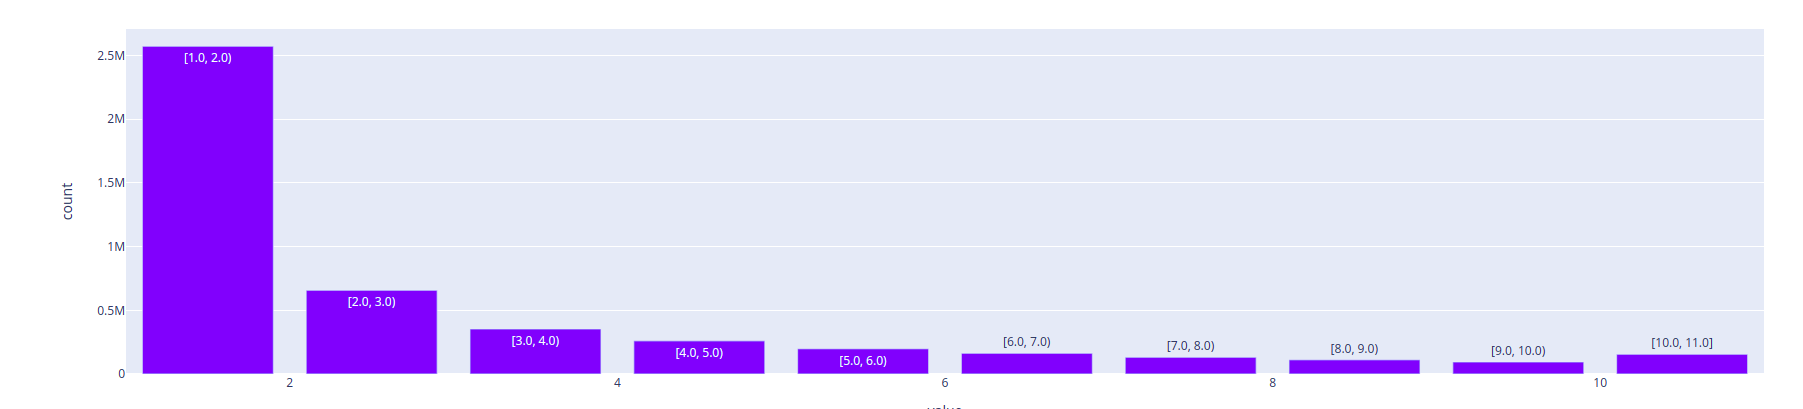
\includegraphics[scale=0.28]{busyPlate.png}

هیستوگرام شمارش دوربین‌ها

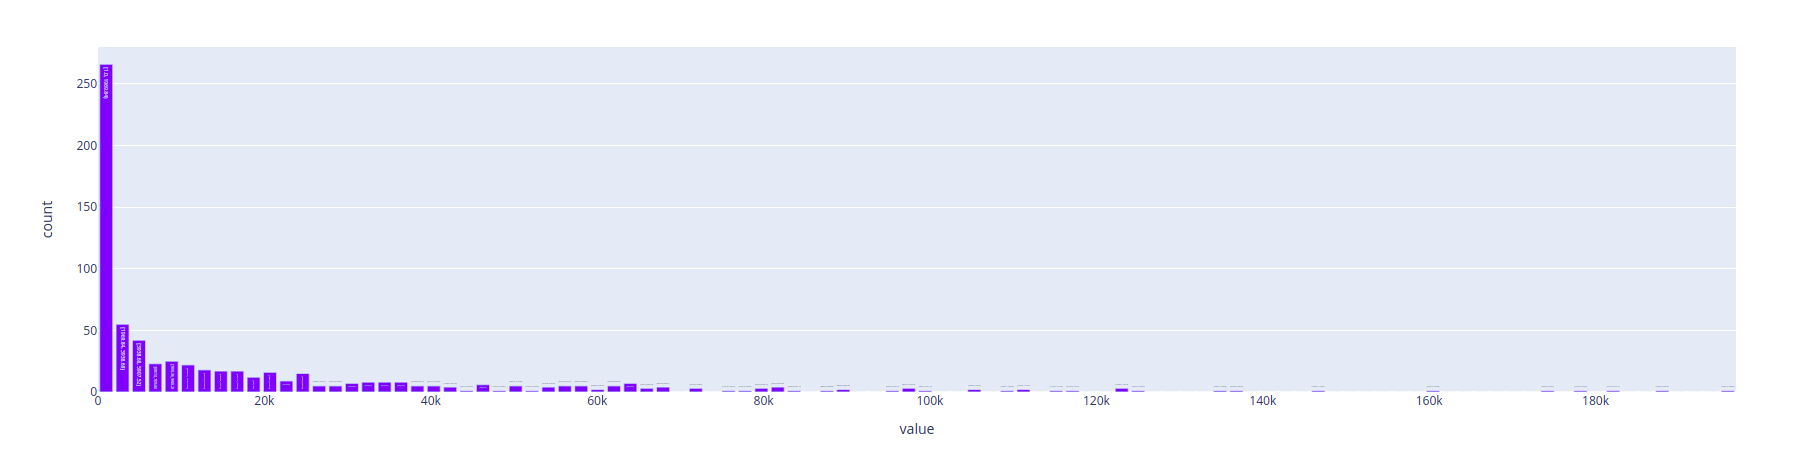
\includegraphics[scale=0.28]{devicePlate.png}

\section*{\lr{Collabarating Filtering}}
در بیش‌تر الگوریتم‌ها هدف بهینه‌بودن کد و تا جای ممکن داشتن زمان مناسب بوده‌است.
برای اینکار سعی شده از توابع آماده خود 
\lr{pyspark}
استفاده کنم چون درغیراینصورت بسیار کند خواهد بود و الگوریتم منطقی نخواهد بود؛ زیرا مسئله زمان پردازش در داده‌های حجیم زیر سوال می‌رود.

با کمی جست‌و‌جو به الگوریتم 
\lr{ALS}
در اسپارک می‌رسیم که با استفاده از کم‌ترین مربعات و یادگیری ماشین سعی بر پیاده‌سازی سریع الگوریتم 
\lr{CF}
را دارد. در این الگوریتم پلاک‌ها حکم کاربر‌ها و 
دوربین‌ها حکم آیتم‌ها را برای ما دارند و تعداد باری که هم را دیده‌اند حکم امتیازی که یک پلاک به یک آیتم می‌دهد را دارد.
داده‌ها را به دو بخش تمرین و تست تقسیم می‌کنیم و سپس سعی می‌کنیم الگوریتم را اجرا کنیم.
مقدار خطای آن 92.0 بوده‌است. در ادامه چندتا از پیش‌بینی‌ها برای
داده‌های تست را نشان‌داده‌ام و سپس برای هر دوربین چند پلاک که حتما می‌بیندش با پیشبینی تعداد باری که می‌بیند و برای هر‌پلاک چند دوربین
با پیشبینی تعداد باری که می‌بیند را گذاشته‌ام.

\section*{تقسیم داده به بازه‌های ۶ ساعت}
برای گرفتن پیشنهاد با استفاده از بازه‌های ساعتی و پلاک‌ها یا بازه‌های ساعتی و دوربین‌ها نیازمند تبدیل داده‌ها بودیم.
ابتدا روز زمان ثبت را در ستونی ذخیره می‌کردم و سپس ساعت‌ها را با تقسیم بر ۶ کردن به اندیس‌های به خصوصی مپ کردم و با ساختن رشته جدید با چسباندن این دو توانستم رکورد‌ها را با استفاده از
پلاک و دوربین و ساعت و روز به خصوص گروه‌بندی کنم و سپس شمارش را انجام دهم.

از آنجایی که الگوریتم‌هایی که از آن‌ها استفاده می‌کنیم نیازمند یک عدد و نه رشته برای هرکدام بود باید آن‌ها به ایندکسی مپ می‌کردم.
سپس یک بار توسط پلاک و زمان و بار دیگر توسط دوربین و زمان گروه‌بندی کرده‌ام و شمارش کردم.

\section*{\lr{Colaberating Filtering Per 6 Hour}}
\subsection*{Device}
همان الگوریتمی که در بخش‌های قبل توضیح داده‌ام را استفاده می‌کنیم. با این
تفاوت که کاربر‌ها همان دوربین‌ها هستند و آیتم‌ها بازه‌های ساعتی ۶ ساعته هستند.
\subsection*{Plate}
همان الگوریتمی که در بخش‌های قبل توضیح داده‌ام را استفاده می‌کنیم. با این
تفاوت که کاربر‌ها همان پلاک‌ها هستند و آیتم‌ها بازه‌های ساعتی ۶ ساعته هستند.

\section*{\lr{Utility Matrix \& SVD}}
بخشی که به شدت چالش برانگیز بود و بسیار نیازمند فکر زیاد بود، ساختن ماتریسی 
\lr{Utility}
از رکورد‌ها بود. خوش‌بختانه با جست‌و‌جو برای مطالب دیگر به طور اتفاقی روشی برای ساخت این ماتریس در زمان معقول پیدا کردم.
ماتریسی که ساخته می‌شود باید هرسطر برای یک پلاک باشد که هراندیس آن نشان‌دهنده تعداد باری است که آن دوربین به خصوص را دیده‌است.
اما برای اینکار یک سری از زوج‌های دوربین‌ها و پلاک‌ها را نداشتیم و باید کراس می‌کردیم و اینگونه
داده اضافی تولید می‌شد. همچنین برای ساخت بردار باید ترتیب‌ها در همه
سطر‌ها درست باشد و به عبارتی باید تابع سورت را اجرا می‌کردیم که باعث زیاد شدن زمان اجرا می‌شد.
بنابراین از ایندکس‌گذاری روی تمام دوربین‌ها و همچنین طریقه ساخت بردار اسپارس کمک گرفتم و
برای هررکورد ایندکس دوربین را به تعداد باری که دیده‌شده مپ کردم و سپس با استفاده از پلاک گروه‌بندی کردم و 
توسط این مپ‌ها بردار اسپارس را ساختم. البته راه آسان‌تر که بعدا به ذهنم رسید این بود که یک لیست از ایندکس‌ها و یک لیست از شمارش‌ها بسازم و آن‌دو را به بردار
اسپارس بدهم تا برایم بسازد.
حال که بردار‌ها را داریم کافیست که آن را به 
\lr{RowMatrix}
بدهیم تا بتوانیم از طریق آن 
\lr{svd}
آن را محاسبه کنیم.

پس از محاسبه ماتریس را بر بردار‌های 
\lr{$V \& U$}
ضرب کردم اما هیچ نتیجه خاصی پیدا نکردم. همچنین همین‌کار را با تعداد فاکتور‌های متفاوت کردم و نتوانستم به داده مناسب خوبی برسم. فاکتور‌ها ۵ و ۱۰ و ۱۵ و ۲۰ را امتحان کردم.

\section*{Clustering}
با استفاده از برداری که بدست آورده‌ایم کلاستر کردن داده‌ها نیز ساده خواهد بود اما چون الگوریتمی که از آن استفاده می‌کنیم برای 
پکیچ یادگیری ماشین است باید بردار همان را استفاده کنیم برای همین بردار‌ها به بردار یادگیری ماشین تبدیل کرده‌ام.

البته شایان ذکر است که در این بخش آن‌قدر کار نکرده‌ام و چیز زیادی برای ارائه ندارم. تنها از الگوریتم دریکله که در کلاس ارائه شده استفاده کرده‌ام و سعی کردم تاپیک‌ها را برای هربخش بدست آوردم
اما از آنجایی که نتوانستم شهود خوبی در بخش 
\lr{svd}
روی فاکتور‌ها پیدا کنم، در این قسمت نیز شکست خوردم و تحقیق بیشتر را بعد از 
نتیجه گرفتن در 
\lr{svd}
گذاشته‌ام که متاسفانه به آن هم نرسیدم.

\section*{مسائل مربوط به گراف}
پس از آن سعی کردم الگوریتم‌های گرافی را تست کنم و سعی کنم اطلاعات با‌ارزشی بدست آوردم اما متاسفانه
با سرچ متوجه شدم که پکیج
\lr{graphx}
در اسپارک جدید است و تنها اسکالا آن را ساپورت می‌کند و برای همین باید با اسکالا پیاده‌سازی می‌شد.
اما متاسفانه به دلیل مشکلات شخصی مانند اوایل نتوانستم روی پروژه کار کنم و روی اسکالا ادامه ندادم.

البته به این هم فکر کردم که خودم آن را روی پایتون خام پیاده‌سازی کنم اما هم حلقه  در پایتون کند است و 
هم داده‌ها بسیار زیاد است و این‌کار منطقی نبود. چون پیاده‌سازی آن‌ها آنقدر سخت نبود و همانطور که اجازه داده بودید به شخصه ظرف چند دقیقه با کد برای یکی از سوال‌ها کد آن را زدم ولی هدف پیاده‌سازی برای داده‌های حجیم بود که اینکار در پایتون و بدون کتاب‌خانه درست منطقی نبود.

\section*{Streaming}
در این بخش الگوریتمی روی داده‌ها برای ارائه ندارم و صرفا کد‌هایی که با آن‌ها روی مسلط شدن بر بخش استریم اسپارک کار می‌کردم قرار دارد.
دلیل اینکه به مشکل خوردم این بود که وقتی یک کد را اسپارک اجرا می‌کند تمام آن بخش با تمام حافظه را بین تمام ورکر‌ها کپی می‌کند و موازی جلو می‌برند؛ بنابراین
در زمان استریم اگر یک دیکشنری که برای هر ای‌دی نگه داشته که چند‌بار دیده را ذخیره کرده باشیم، در زمان آمدن داده‌های جدید دیکشنری ریست می‌شود و به مقدار اولیه قبل از اجرای کد می‌رود و به همین دلیل شمارش اشتباهی صورت می‌گیرد و به همین منظور برای هر‌داده نمی‌توانیم نگه داریم که چندمین بار است که دیده می‌شود و به همین دلیل نمی‌توانیم مومنت‌ها را بشماریم.
\end{document}


